
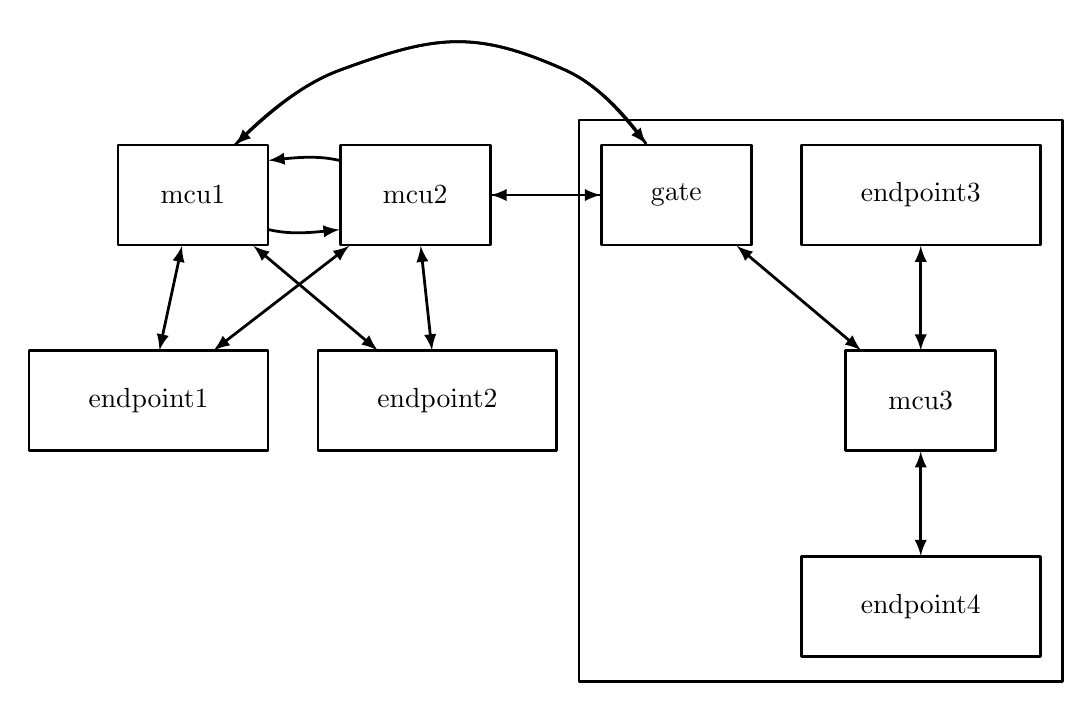
\begin{tikzpicture}[>=latex,line join=bevel,]
  \pgfsetlinewidth{1bp}
%%
\begin{scope}
  \pgfsetstrokecolor{black}
  \definecolor{strokecol}{rgb}{0.0,0.0,0.0};
  \pgfsetstrokecolor{strokecol}
  \draw (198bp,8bp) -- (198bp,210bp) -- (372bp,210bp) -- (372bp,8bp) -- cycle;
\end{scope}
  \pgfsetcolor{black}
  % Edge: gate -> mcu2
  \draw [->] (205.85bp,183bp) .. controls (196.03bp,183bp) and (186.22bp,183bp)  .. (166.17bp,183bp);
  % Edge: gate -> mcu1
  \draw [->] (222.15bp,201.39bp) .. controls (215.21bp,211.27bp) and (205.21bp,222.52bp)  .. (193bp,228bp) .. controls (160.16bp,242.75bp) and (145.79bp,240.41bp)  .. (112bp,228bp) .. controls (100.72bp,223.86bp) and (90.203bp,216.13bp)  .. (74.174bp,201.04bp);
  % Edge: mcu2 -> mcu1
  \draw [->] (111.77bp,195.46bp) .. controls (106.57bp,196.61bp) and (101.38bp,197.06bp)  .. (86.188bp,195.45bp);
  % Edge: endpoint3 -> mcu3
  \draw [<->] (321bp,164.71bp) .. controls (321bp,149.05bp) and (321bp,143.12bp)  .. (321bp,127.08bp);
  % Edge: mcu3 -> endpoint4
  \draw [<->] (321bp,90.708bp) .. controls (321bp,75.053bp) and (321bp,69.116bp)  .. (321bp,53.082bp);
  % Edge: mcu1 -> mcu2
  \draw [->] (86.188bp,170.55bp) .. controls (91.384bp,169.39bp) and (96.58bp,168.94bp)  .. (111.77bp,170.54bp);
  % Edge: mcu1 -> endpoint2
  \draw [<->] (80.753bp,164.71bp) .. controls (97.813bp,150.36bp) and (108.19bp,141.64bp)  .. (125.5bp,127.08bp);
  % Edge: mcu2 -> endpoint2
  \draw [<->] (140.98bp,164.71bp) .. controls (142.69bp,148.91bp) and (143.34bp,142.81bp)  .. (145.05bp,127.08bp);
  % Edge: mcu2 -> endpoint1
  \draw [<->] (115.27bp,164.71bp) .. controls (96.758bp,150.44bp) and (85.07bp,141.43bp)  .. (66.457bp,127.08bp);
  % Edge: mcu2 -> gate
  \draw [->] (166.17bp,183bp) .. controls (175.99bp,183bp) and (185.8bp,183bp)  .. (205.85bp,183bp);
  % Edge: mcu1 -> gate
  \draw [->] (74.174bp,201.04bp) .. controls (83.833bp,211.07bp) and (97.27bp,222.59bp)  .. (112bp,228bp) .. controls (145.79bp,240.41bp) and (160.16bp,242.75bp)  .. (193bp,228bp) .. controls (201.96bp,223.97bp) and (209.74bp,216.84bp)  .. (222.15bp,201.39bp);
  % Edge: mcu1 -> endpoint1
  \draw [<->] (55.045bp,164.71bp) .. controls (51.629bp,148.91bp) and (50.311bp,142.81bp)  .. (46.91bp,127.08bp);
  % Edge: gate -> mcu3
  \draw [<->] (254.75bp,164.71bp) .. controls (271.81bp,150.36bp) and (282.19bp,141.64bp)  .. (299.5bp,127.08bp);
  % Node: mcu3
\begin{scope}
  \definecolor{strokecol}{rgb}{0.0,0.0,0.0};
  \pgfsetstrokecolor{strokecol}
  \draw (294bp,91bp) -- (294bp,127bp) -- (348bp,127bp) -- (348bp,91bp) -- cycle;
  \draw (321bp,109bp) node {mcu3};
\end{scope}
  % Node: endpoint1
\begin{scope}
  \definecolor{strokecol}{rgb}{0.0,0.0,0.0};
  \pgfsetstrokecolor{strokecol}
  \draw (0bp,91bp) -- (0bp,127bp) -- (86bp,127bp) -- (86bp,91bp) -- cycle;
  \draw (43bp,109bp) node {endpoint1};
\end{scope}
  % Node: gate
\begin{scope}
  \definecolor{strokecol}{rgb}{0.0,0.0,0.0};
  \pgfsetstrokecolor{strokecol}
  \draw (206bp,165bp) -- (206bp,201bp) -- (260bp,201bp) -- (260bp,165bp) -- cycle;
  \draw (233bp,183bp) node {gate};
\end{scope}
  % Node: endpoint2
\begin{scope}
  \definecolor{strokecol}{rgb}{0.0,0.0,0.0};
  \pgfsetstrokecolor{strokecol}
  \draw (104bp,91bp) -- (104bp,127bp) -- (190bp,127bp) -- (190bp,91bp) -- cycle;
  \draw (147bp,109bp) node {endpoint2};
\end{scope}
  % Node: endpoint3
\begin{scope}
  \definecolor{strokecol}{rgb}{0.0,0.0,0.0};
  \pgfsetstrokecolor{strokecol}
  \draw (278bp,165bp) -- (278bp,201bp) -- (364bp,201bp) -- (364bp,165bp) -- cycle;
  \draw (321bp,183bp) node {endpoint3};
\end{scope}
  % Node: endpoint4
\begin{scope}
  \definecolor{strokecol}{rgb}{0.0,0.0,0.0};
  \pgfsetstrokecolor{strokecol}
  \draw (278bp,17bp) -- (278bp,53bp) -- (364bp,53bp) -- (364bp,17bp) -- cycle;
  \draw (321bp,35bp) node {endpoint4};
\end{scope}
  % Node: mcu2
\begin{scope}
  \definecolor{strokecol}{rgb}{0.0,0.0,0.0};
  \pgfsetstrokecolor{strokecol}
  \draw (112bp,165bp) -- (112bp,201bp) -- (166bp,201bp) -- (166bp,165bp) -- cycle;
  \draw (139bp,183bp) node {mcu2};
\end{scope}
  % Node: mcu1
\begin{scope}
  \definecolor{strokecol}{rgb}{0.0,0.0,0.0};
  \pgfsetstrokecolor{strokecol}
  \draw (32bp,165bp) -- (32bp,201bp) -- (86bp,201bp) -- (86bp,165bp) -- cycle;
  \draw (59bp,183bp) node {mcu1};
\end{scope}
%
\end{tikzpicture}

